After the stress-test, when the transactions and operations had been added to
the blockchain, we reviewed the blockchain off-line. Given
that the transactions and operations are recorded on the blockchain, we
started by investigatng the overall results first.

As can be seen from \cref{fig:tpsall} (top), there are multiple periods of
activity. Clearly, most of the transactions started being
broadcast from 15:00 going forward with an average of approximately
\SI{1000}{transactions per block} afterwards. We also notice that the
throughput was not constant during the stress-test which can be explained by the
transactions requiring some time to propagate through the Peer-2-Peer network.

We can further see in \cref{fig:tpsall} (bottom), that the participants have
been constantly trying to modify their spam production method (increaseing number
of transactions vs.\ bundling more operations per transaction) until a maximum
of processed operations per block was reached at about 16:40. Afterwards, the
participants were asked to increase the number of created transactions
instead which is why the processed operations per block decreased later on.

\begin{figure}[!htp]
 \centering
 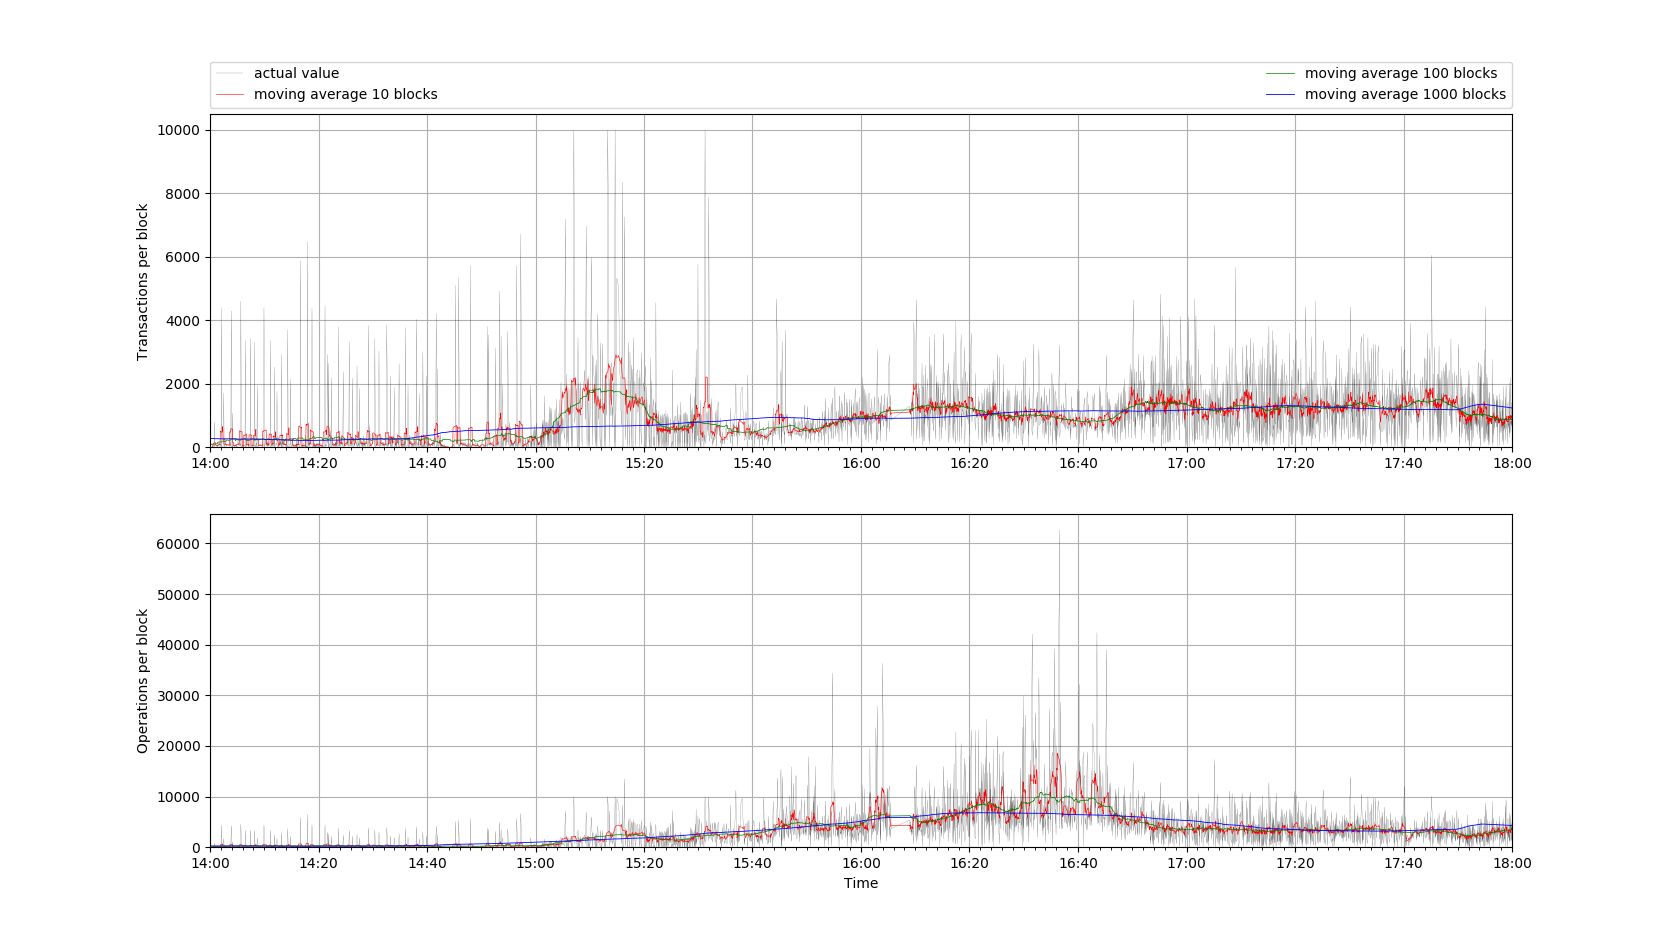
\includegraphics[width=\linewidth]{figures/stress-test-overview.png}
 \caption{Overview of the throughput ops/s and txs/s during the whole stress-test}
 \label{fig:tpsall}
\end{figure}

Most interestingly, we observed several short peaks of processed transactions and
operations during the whole stress-test. As it turned out, the reasons of those
peaks can be explained by a single participant who decided to use his
block validating node to produce transactions. By this, he skipped the
propagation of transactions through the Peer-2-Peer network which confirms to
us that the networking code represents one of the bottlenecks.

\begin{figure}[!htp]
 \centering
 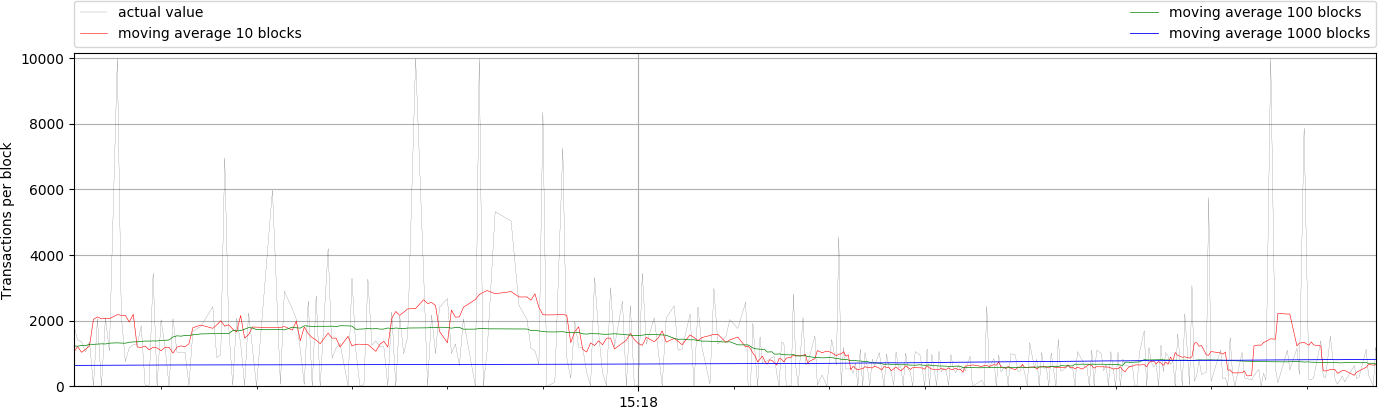
\includegraphics[width=\linewidth]{figures/stress-test-max-tps.png}
 \caption{Max ops/s during the stress-test}
 \label{fig:tps}
\end{figure}

In \cref{fig:tps}, we have zoomed into a period of rather high throughput (i.e.
\SI{2500}{transactions per block}). Here, we still see the peaks produced by
skipping the networking.

\begin{figure}[!htp]
 \centering
 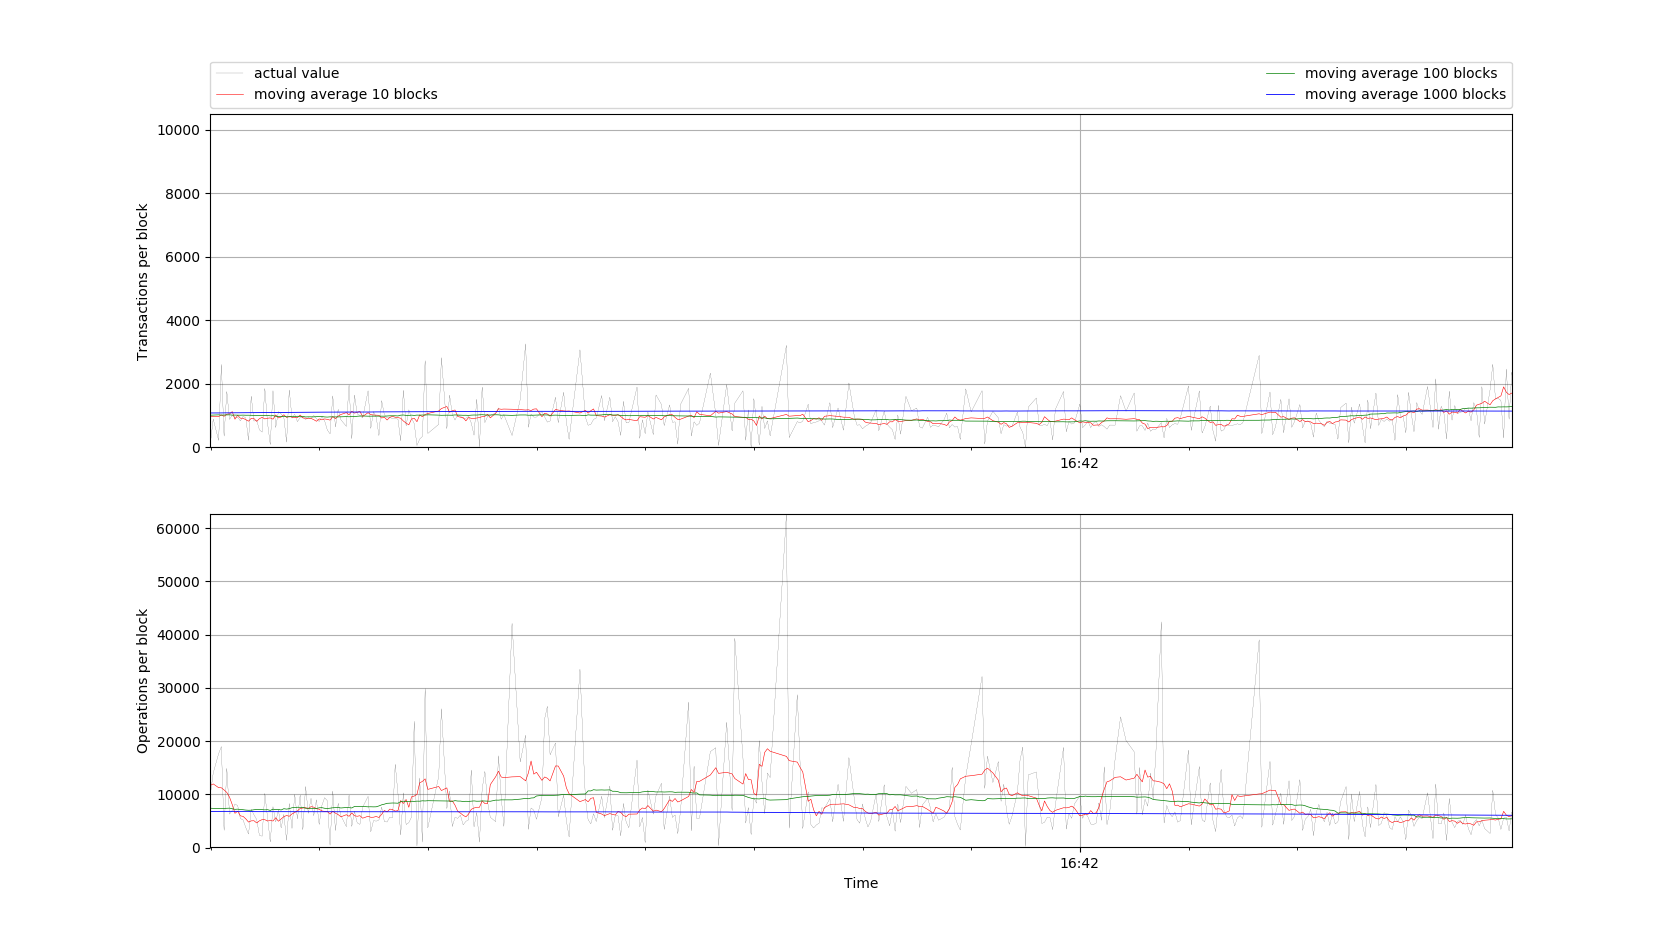
\includegraphics[width=\linewidth]{figures/stress-test-max-ops.png}
 \caption{Max ops/s during the stress-test}
 \label{fig:ops}
\end{figure}

Finally, the results in \cref{fig:ops} show that the blockchain was able to
process an average of over \SI{8000}{operations per block} with quite high
peaks and an irregular throughput per block.

\begin{figure}[!htp]
 \centering
 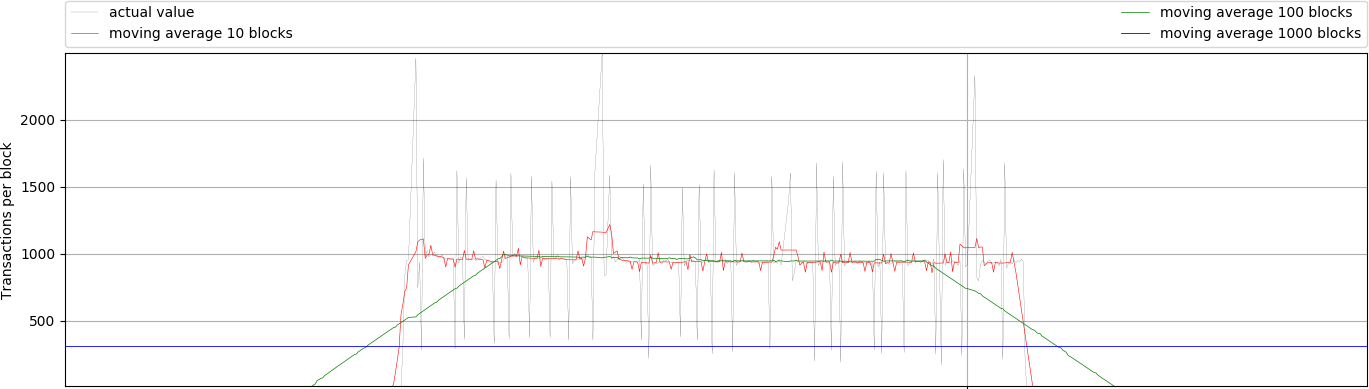
\includegraphics[width=\linewidth]{figures/stress-test-constant-load.png}
 \caption{Max ops/s during the stress-test}
 \label{fig:ops-const}
\end{figure}

The irregularity can be resolved by deploying similar hardware that can all
process the same amount of transactions/operations. We were able to confirm
this behavior later on by replacing all validators except for one, which
greatly reduces the variance of the throughput as can be seen in
\cref{fig:ops-const}. Here, the stress has been produce by a single node
connected directly to the validating node while another single validator was
only connected through the Peer-2-Peer network.
